\subsection{\label{sec:stellarium}Stellarium}

In order to check the validity of our livestream-derived optical lightcurve, we needed a way of finding the expected eclipse obscuration percentage over time for our location.
We used the free, open-source planetarium software \texttt{Stellarium}\cite{zotti_simulated_2020} to achieve this.
After setting the time, date, and location of our radio telescope in \texttt{Stellarium}, we queried the software's API to step the simulation time forward and extracted the eclipse percentage for 1000 points in time, starting before first contact and ending after fourth contact.
The resulting theoretical lightcurve was then overlaid on the eclipse obscuration derived from the UCA Observatory livestream.
The agreement between the two is excellent, as shown in Figure \ref{fig:LightcurveComparison}, validating our optical eclipse lightcurve.

\subsection{\label{sec:theoreticalLightcurves}Theoretical Lightcurve Comparison}

To determine the apparent radius of the sun at \unit[1420]{MHz}, we compared our observed radio lightcurve to a series of theoretical lightcurves where the radius of the sun has been changed.
To accomplish this, we first downloaded high-accuracy ephemeris data from the JPL Horizons On-Line Ephemeris System \cite{nasa_jpl_solar_system_dynamics_group_jpl_nodate}. 
Using the angular radii of both the sun and moon along with the angular separation between the two, we calculated the obscured area of the solar disk at 2000 points in time during the eclipse using the geometric relationships shown in Figure \ref{fig:eclipse_geometry}.
These relationships are also given by Equations \ref{eq:geometry_1} through \ref{eq:geometry_4}.

\begin{figure}
\begin{minipage}{0.49\textwidth}
  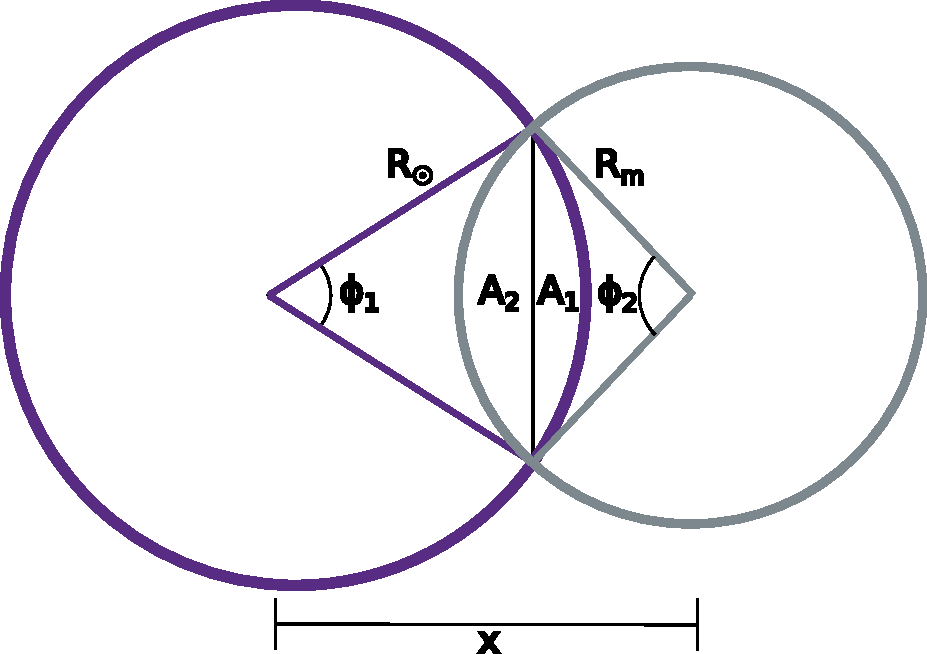
\includegraphics[width=0.75\textwidth]{figures/drawing_updated}
  \caption{\label{fig:eclipse_geometry} The geometric relationships used to calculate the obscuration of the sun. The percent obscuration is found by dividing the combined area $A_1 + A_2$ by the apparent area of the sun's disk $\pi R_\odot^2$}
\end{minipage}
\hfill
\begin{minipage}{0.49\textwidth}
\begin{equation}\label{eq:geometry_1}
  A_1 = \frac{1}{2}R_{\odot}^2\left(\phi_1 - \sin\phi_1\right)
\end{equation}
\begin{equation}\label{eq:geometry_2}
  A_2 = \frac{1}{2}R_{m}^2\left(\phi_2 - \sin\phi_2\right)
\end{equation}
\begin{equation}\label{eq:geometry_3}
  \phi_1 = 2\cos^{-1}\left(\frac{R_{\odot}^2 - R_{m}^2+x^2}{2R_{\odot}x}\right)
\end{equation}
\begin{equation}\label{eq:geometry_4}
  \phi_2 = 2\cos^{-1}\left(\frac{x^2 - R_{\odot}^2 + r_{m}^2}{2R_{m}x}\right)
\end{equation}
\end{minipage}
\end{figure}



\begin{figure}
  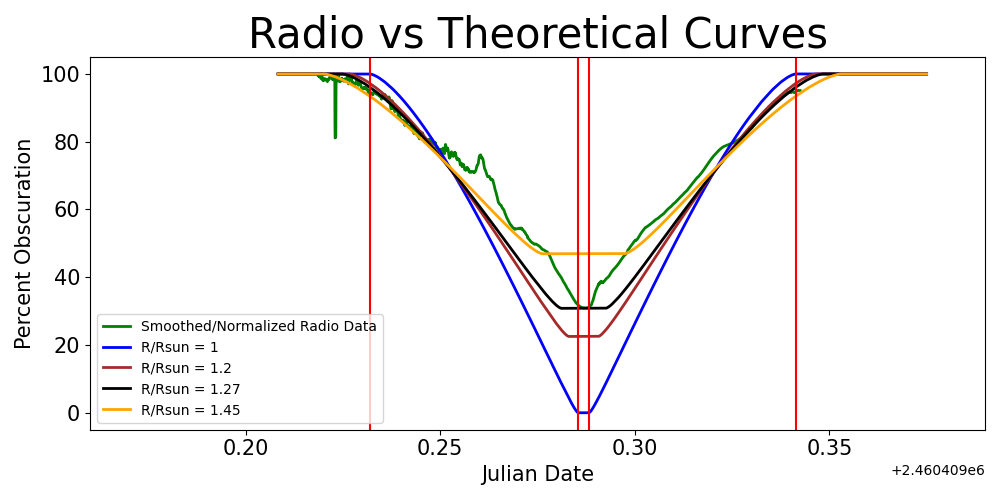
\includegraphics[width=0.93\textwidth]{figures/RadiovsTheoretical}
  \caption{\label{fig:RadiovsTheoretical} A comparison of the smoothed/normalized radio lightcurve and theoretical lightcurves generated with the JPL Horizons ephemeris data. Our best fit to the depth of the radio lightcurve has an apparent solar radius of $1.27 R_{\odot}$}
\end{figure}

Our data found that the radio lightcurve reached a minimum of 30.9\% of the total solar flux during totality.
Using these relationships, we were able to create theoretical lightcurves for varying solar radii from $R = 1.0 R_{\odot}$ to $R = 1.45 R_{\odot}$.
We found our best-fitting solar raius by manually adjusting the model until the difference between the observed and model minima dropped below 1\%.

These theoretical lightcurves, shown in Figure \ref{fig:RadiovsTheoretical}, helped us match the dip in relative brightness within the radio lightcurve, but it was not a perfect match.
Although the dip in brightness was accurate, the curves show variance in slope and our radio data does not show the flat bottom expected while the moon transits the larger solar disk.
The theoretical curves assume a uniform disk brightness, not accounting for limb darkening, sunspots, radio emission from the corona, or other solar activity.
Despite these variances, we found that the best-fit curve has an apparent solar radius of $R_{\mathrm{1420}} = 1.27 R_{\odot}$.
This lies between the results of $R_{\mathrm{1420}} = 1.14 R_{\odot}$ found by \cite{messerotti_radio_2000}, and $R_{\mathrm{1420}} = 1.4 R_{\odot}$ found by \cite{leung_solar_2022}.
Both of these references observed partial solar eclipses at \unit[1420]{MHz}. In the case of \cite{leung_solar_2022}, those observations were made with the same radio receiver and software used in this study.


Our results are consistent with the trend found in \cite{menezes_solar_2017}, which compared decades of solar radio observations taken at many wavelengths, and found that solar radius increased as the radio frequency decreased (their Figure 5 and Equation 2).
This was also seen in the results of \cite{messerotti_radio_2000}, which observed the eclipse at four different wavelengths and found a similar trend (their Table 2.)





